\documentclass[11pt]{article}
 
\usepackage[margin=.95in]{geometry} 
\usepackage{amsmath,amsthm,amssymb, graphicx, multicol, array}
 
\newcommand{\N}{\mathbb{N}}
\newcommand{\Z}{\mathbb{Z}}
 

\begin{document}
 
\title{Homework 2}
\author{Juliette Franqueville\\
}
\maketitle

\subsection*{(1)  For $y_1,.., y_n \sim \mathcal{N}(\mu,\sigma^2 )$, show that $s = (\bar{y},s^2 )$ are sufficient. Also, find the observed and the expected information matrices}

The factorization theorem says that statistic $s$ is sufficient iif $f(y_{1:n}|\theta) = g(s|\theta)h(y_{1:n})$. For the normal, we have:

\begin{align*}
   f(y_{1:n}|\theta) &= \prod (2\pi \sigma^2)^{-1/2} \text{exp}\left(-\frac{(y_i-\mu)^2}{2\sigma^2}\right) \\
   &=(2\pi \sigma^2)^{-n/2}\text{exp}\left(-\frac{\sum (y_i-\mu)^2}{2\sigma^2}\right) \\
    &=(2\pi \sigma^2)^{-n/2}\text{exp}\left(-\frac{\sum ([y_i-\bar{y}]-[\mu-\bar{y})]^2}{2\sigma^2}\right) \\
    &=(2\pi \sigma^2)^{-n/2}\text{exp}\left(-\frac{\sum \{ [y_i-\bar{y}]^2-2[y_i-\bar{y}][\mu-\bar{y}]+[\mu-\bar{y}]^2 \}}{2\sigma^2}\right) \\
        &=(2\pi \sigma^2)^{-n/2}\text{exp}\left(-\frac{\sum \{ [y_i-\bar{y}]^2+[\mu-\bar{y}]^2 \}}{2\sigma^2}\right) \\
        &=(2\pi \sigma^2)^{-n/2}\text{exp}\left(-\frac{\sum  [y_i-\bar{y}]^2}{2\sigma^2}\right) \text{exp}\left(-\frac{n [\mu-\bar{y}]^2}{2\sigma^2}\right) \\
        &=(2\pi \sigma^2)^{-n/2}\text{exp}\left(-\frac{\sum  [y_i-\bar{y}]^2}{2\sigma^2}\right) \text{exp}\left(-\frac{n [\mu-\bar{y}]^2}{2\sigma^2}\right) \\
    &=(2\pi \sigma^2)^{-n/2}\text{exp}\left(-\frac{(n-1)s^2}{2\sigma^2}\right) \text{exp}\left(-\frac{n [\mu-\bar{y}]^2}{2\sigma^2}\right) \\
\end{align*}


We recognize $h(y_{1:n}) =1 $ and $g(\bar{y}, s^2|\mu, \sigma^2)= (2\pi \sigma^2)^{-n/2}\text{exp}\left(-\frac{(n-1)s^2}{2\sigma^2}\right) \text{exp}\left(-\frac{n [\mu-\bar{y}]^2}{2\sigma^2}\right)$ is a sufficient statistic for $(\mu, \sigma^2)$.

The observed information matrix, $-\frac{\partial \mathcal{L}(\boldsymbol{\theta})}{\boldsymbol{\theta}^T \boldsymbol{\theta}}$, is:
\begin{center}
    \begin{bmatrix}

\frac{n}{\sigma^2} & \frac{n(\bar{y}-\mu)}{\sigma^4} \\
 \frac{n(\bar{y}-\mu)}{\sigma^4}  & \frac{n}{2\sigma^4} + \frac{1}{\sigma^6}\sum(y_i-\mu)^2)
\end{bmatrix}
\end{center}
and the expected information matrix, $E\left(-\frac{\partial \mathcal{L}(\boldsymbol{\theta})}{\boldsymbol{\theta}^T \boldsymbol{\theta}}\right)$



\begin{center}
    \begin{bmatrix}

\frac{n}{\sigma^2} & 0\\
0 & \frac{n}{2\sigma^4} 
\end{bmatrix}
\end{center}


Most terms are evident, except 

\begin{align*}
    E\left[ -\frac{n}{2\sigma^4} + \frac{1}{\sigma^6}\sum(y_i-\mu)^2)\right] &=- \frac{n}{2\sigma^4}+\frac{1}{\sigma^6}E\left(\sum y_i^2-2\mu \sum y_i+n\mu^2\right)\\ &=- \frac{n}{2\sigma^4}+\frac{n}{\sigma^6}[(var(y)+E(y)^2-2\mu E(\bar{y})+\mu^2)]\\
    &=- \frac{n}{2\sigma^4}+\frac{n}{\sigma^6}[\sigma^2+\mu^2-2\mu^2+\mu^2]\\ &=\frac{n}{2\sigma^4}
\end{align*}

\subsection*{(2)   If $Y_1,..., Y_n\overset{\text{iid}}{\sim} N(\mu, c \mu^2)$, where c is a known constant, show that the minimal sufficient statistic for $\mu$ is the same as for the $ N(\mu, c \mu^2)$ distribution. Find the maximum likelihood
estimate of µ and give its large-sample standard error. Show that the distribution of $\bar{Y}^2/S^2$ does not depend on $\mu$.}

First we find the minimal sufficient statistics for $N(\mu, \sigma^2)$. We find:

\begin{align*}
    \frac{f(x)}{f(y)} &= \frac{\exp\left(-\frac{\sum (x-\mu)^2}{2\sigma^2}\right)}{\exp\left(-\frac{\sum (y-\mu)^2}{2\sigma^2}\right)}\\
    &= \exp\left(-\frac{1}{2\sigma^2}[\sum(x-\mu)^2 - \sum(y-\mu)^2]\right)\\
     &= \exp\left(-\frac{1}{2\sigma^2}[\sum x_i^2 - \sum y_i^2 - 2\mu(\sum x_i - \sum y_i)\right)
\end{align*}

The ratio is independent of $\mu$ when $\sum x_i^2 = \sum y_i^2$ and independent of $\sigma^$ when  $\sum x_i^2 = \sum y_i^2$ and  $\sum x_i = \sum y_i$, so $\sum x_i^2$ and $\sum x_i$ are minimally sufficient statistics. Similarly for $N(\mu, c\mu^2)$
\begin{align*}
    \frac{f(x)}{f(y)} 
     &= \exp\left(-\frac{1}{2\mu^2c}[\sum x_i^2 - \sum y_i^2 - 2\mu(\sum x_i - \sum y_i)\right)
\end{align*}

 $\sum x_i^2$ and $\sum x_i$ are minimally sufficient statistics.\\ For  $N(\mu, c\mu^2)$, we have:
 
 \begin{align*}
     L(\mu)  &= \prod (2\pi c\mu^2)^{-1/2} \text{exp}\left(-\frac{(y_i-\mu)^2}{2c\mu^2}\right) \\
   &=(2\pi c\mu^2)^{-n/2}\text{exp}\left(-\frac{\sum (y_i-\mu)^2}{2c\mu^2}\right) \\
   \mathcal{L}(\mu)&= -\frac{n}{2}log(2\pi c) - \frac{n}{2}log(\mu^2) - -\frac{\sum (y_i-\mu)^2}{2c\mu^2}\\
   \frac{\partial  \mathcal{L}(\mu)}{\partial \mu} &= -\frac{n}{\mu} - \frac{1}{c} \left( \frac{\sum x_i}{\mu^2}-\frac{\sum x_i^2}{\mu^3}\right)
 \end{align*}
 Set the derivative to 0:
 \begin{align*}
      -\frac{n}{\mu} - \frac{1}{c} \left( \frac{\sum x_i}{\mu^2}-\frac{\sum x_i^2}{\mu^3}\right) &= 0\\
      -n\mu^2 - \frac{1}{c} ( \sum x_i-\sum x_i^2\mu) &= 0\\
       nc\mu^2 +\sum x_i^2\mu  -   \sum x_i&= 0\\
 \end{align*}
 
 Solving for $\mu$:
 
\begin{align*}
     \mu = \frac{-\sum x_i + [(\sum x_i)^2 + 4nc \sum x_i^2]^{1/2}}{2nc}
 \end{align*}
 
 for $\bar{x} > 0$, and 
 
 \begin{align*}
     \mu = \frac{-\sum x_i - [(\sum x_i)^2 + 4nc \sum x_i^2]^{1/2}}{2nc}
 \end{align*}
 
 otherwise (I checked the signs numerically, as suggested by Dr.\ Sarkar). We can estimate the standard error from the Fisher information matrix (se $= I^{-1/2}$) (which is a scalar here).
 
 \begin{align*}
     \frac{\partial ^2 \mathcal{L}(\mu)}{\partial \mu^2} = \frac{n}{\mu^2}-\frac{1}{c}\left[\frac{3\sum x_i^2}{\mu^4}-\frac{2\sum x_i}{\mu^3}\right] \\
     E\left[\frac{\partial ^2 \mathcal{L}(\mu)}{\partial \mu^2}\right] = \frac{n}{\mu^2}-\frac{1}{c}\left[\frac{3 n(\mu^2c+\mu^2)}{\mu^4}-\frac{2n\mu}{\mu^3}\right] \\
      E\left[\frac{\partial ^2 \mathcal{L}(\mu)}{\partial \mu^2}\right] =  -\frac{n}{\mu^2} (2+1/c)\\
      \text{SE}(\mu) =  [\frac{n}{\mu^2} (2+1/c)]^{-1/2}
 \end{align*}
 
We would plug $\mu_{MLE}$ for $\mu$. Finally, to show that the distribution of $\bar{Y}^2/S^2$ does not depend on $\mu$, we use the fact that $y_i/\mu \sim N(1, c)$. Since $S^2 =  (n-1)^{-1} \sum(x_i-\mu)^2$,  $\bar{Y}^2/S^2$  cannot depend on $\mu$. The figure confirms this using simulated data:


 
\begin{figure}[!h]
    \centering
    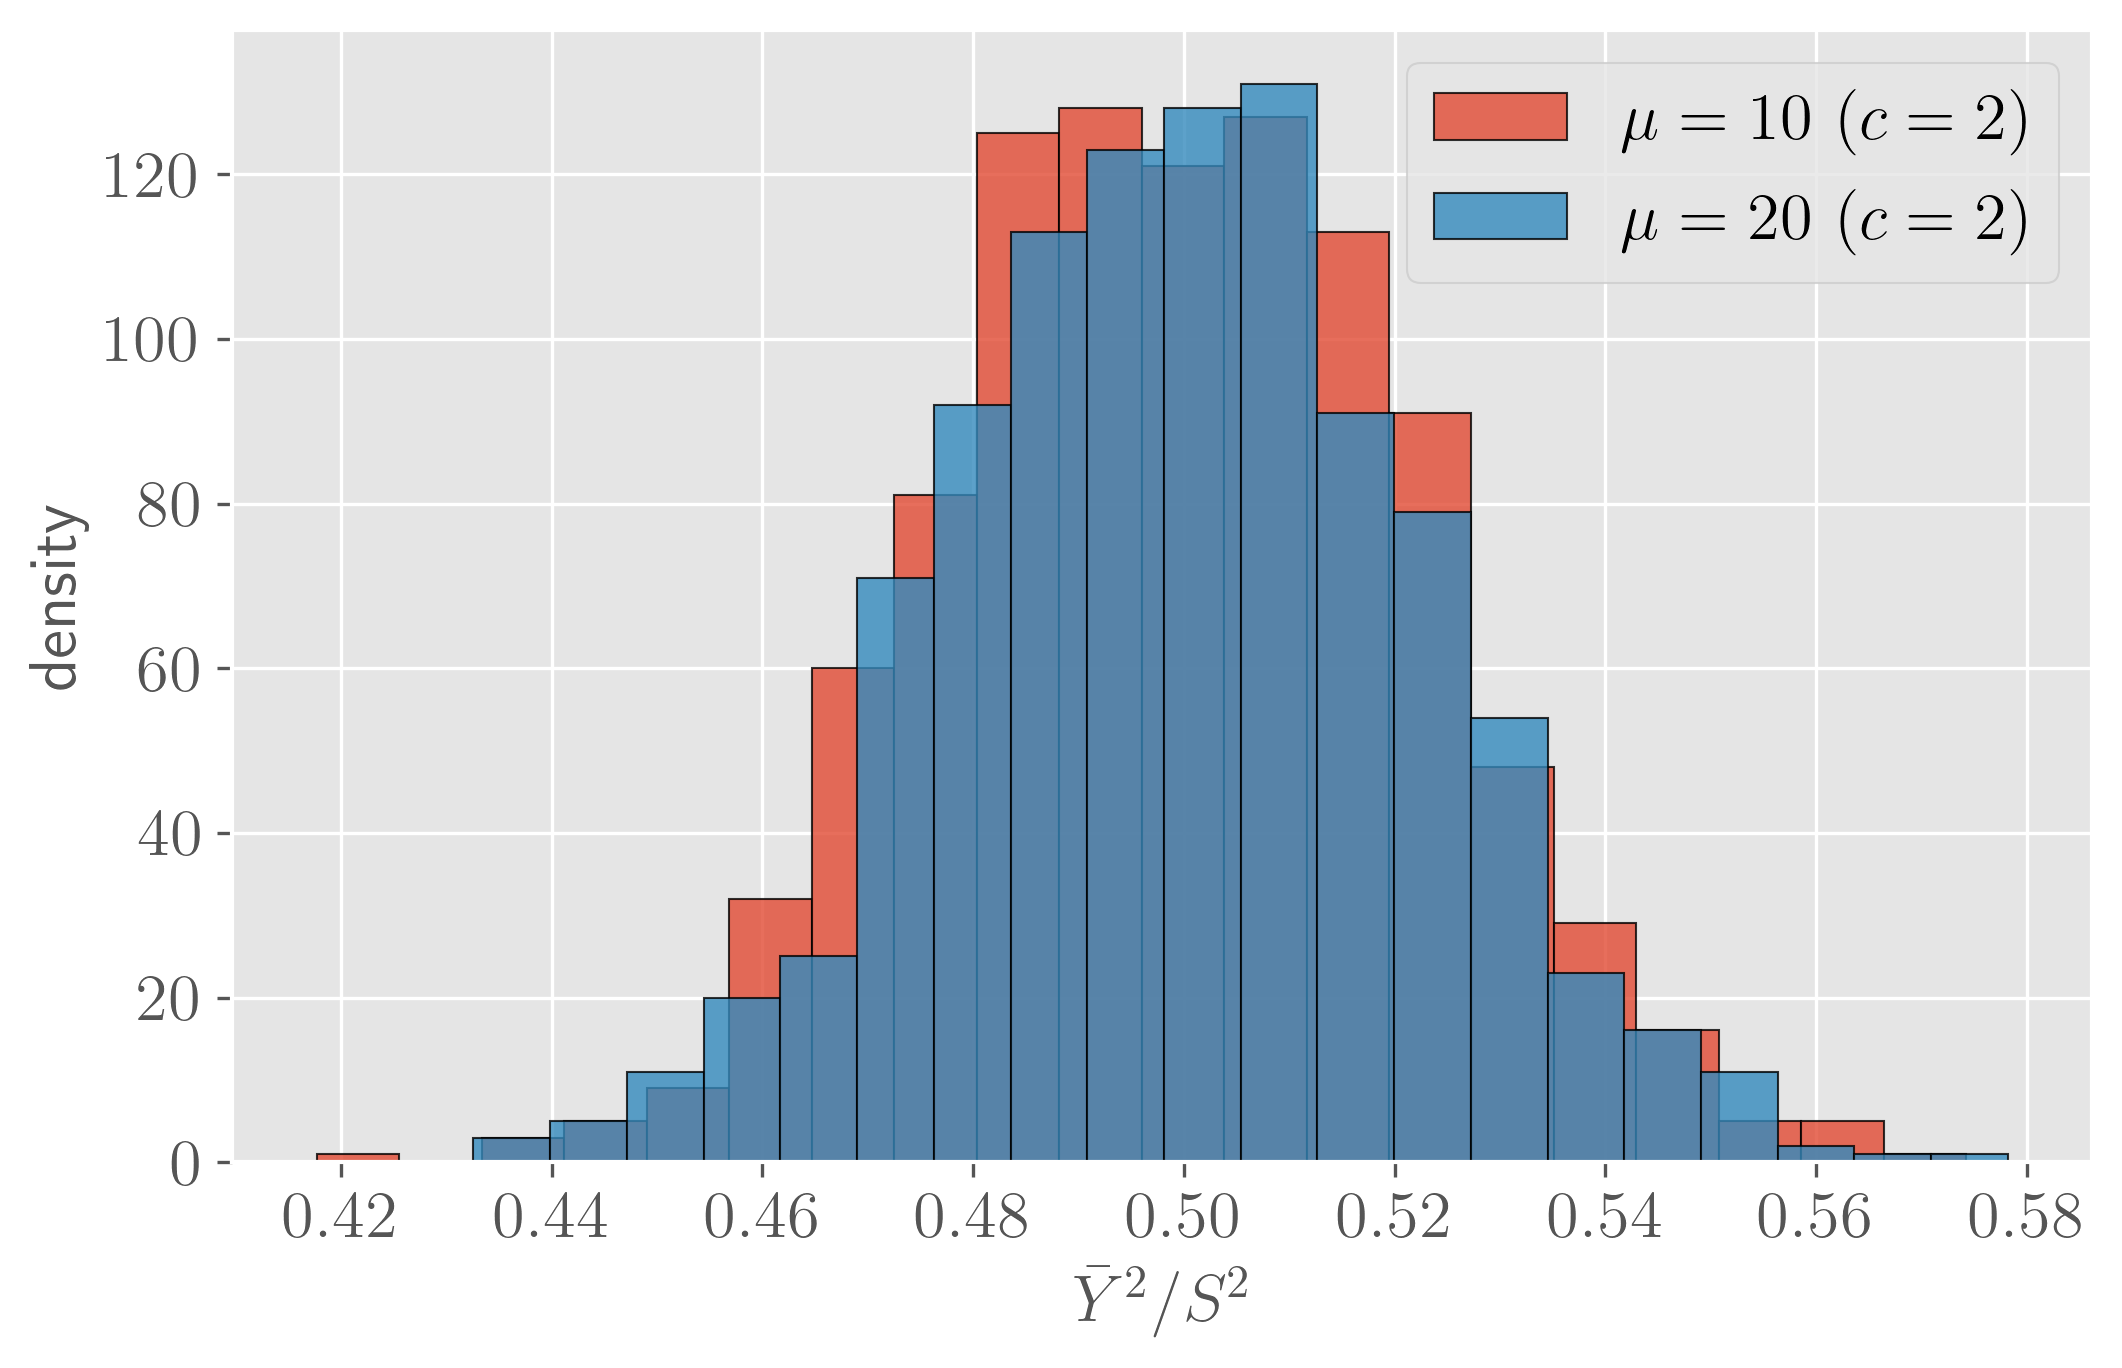
\includegraphics[scale=.55]{homework_2/figures/no_dept.png}
    \caption{Histogram for question (3) (a)}
    \label{fig:my_label}
\end{figure}
 
 
\subsection*{(3)  (a) Draw a random sample of size $n = 2$0 from a $\text{Cauchy}(0,1)$ distribution. Compute $\bar{y}n$. Repeat this $B = 1000$ times. Draw a histogram of the sampled $\bar{y}n$ values, superimposed over a $\text{Cauchy(0,1)}$ density.}

\begin{figure}[!h]
    \centering
    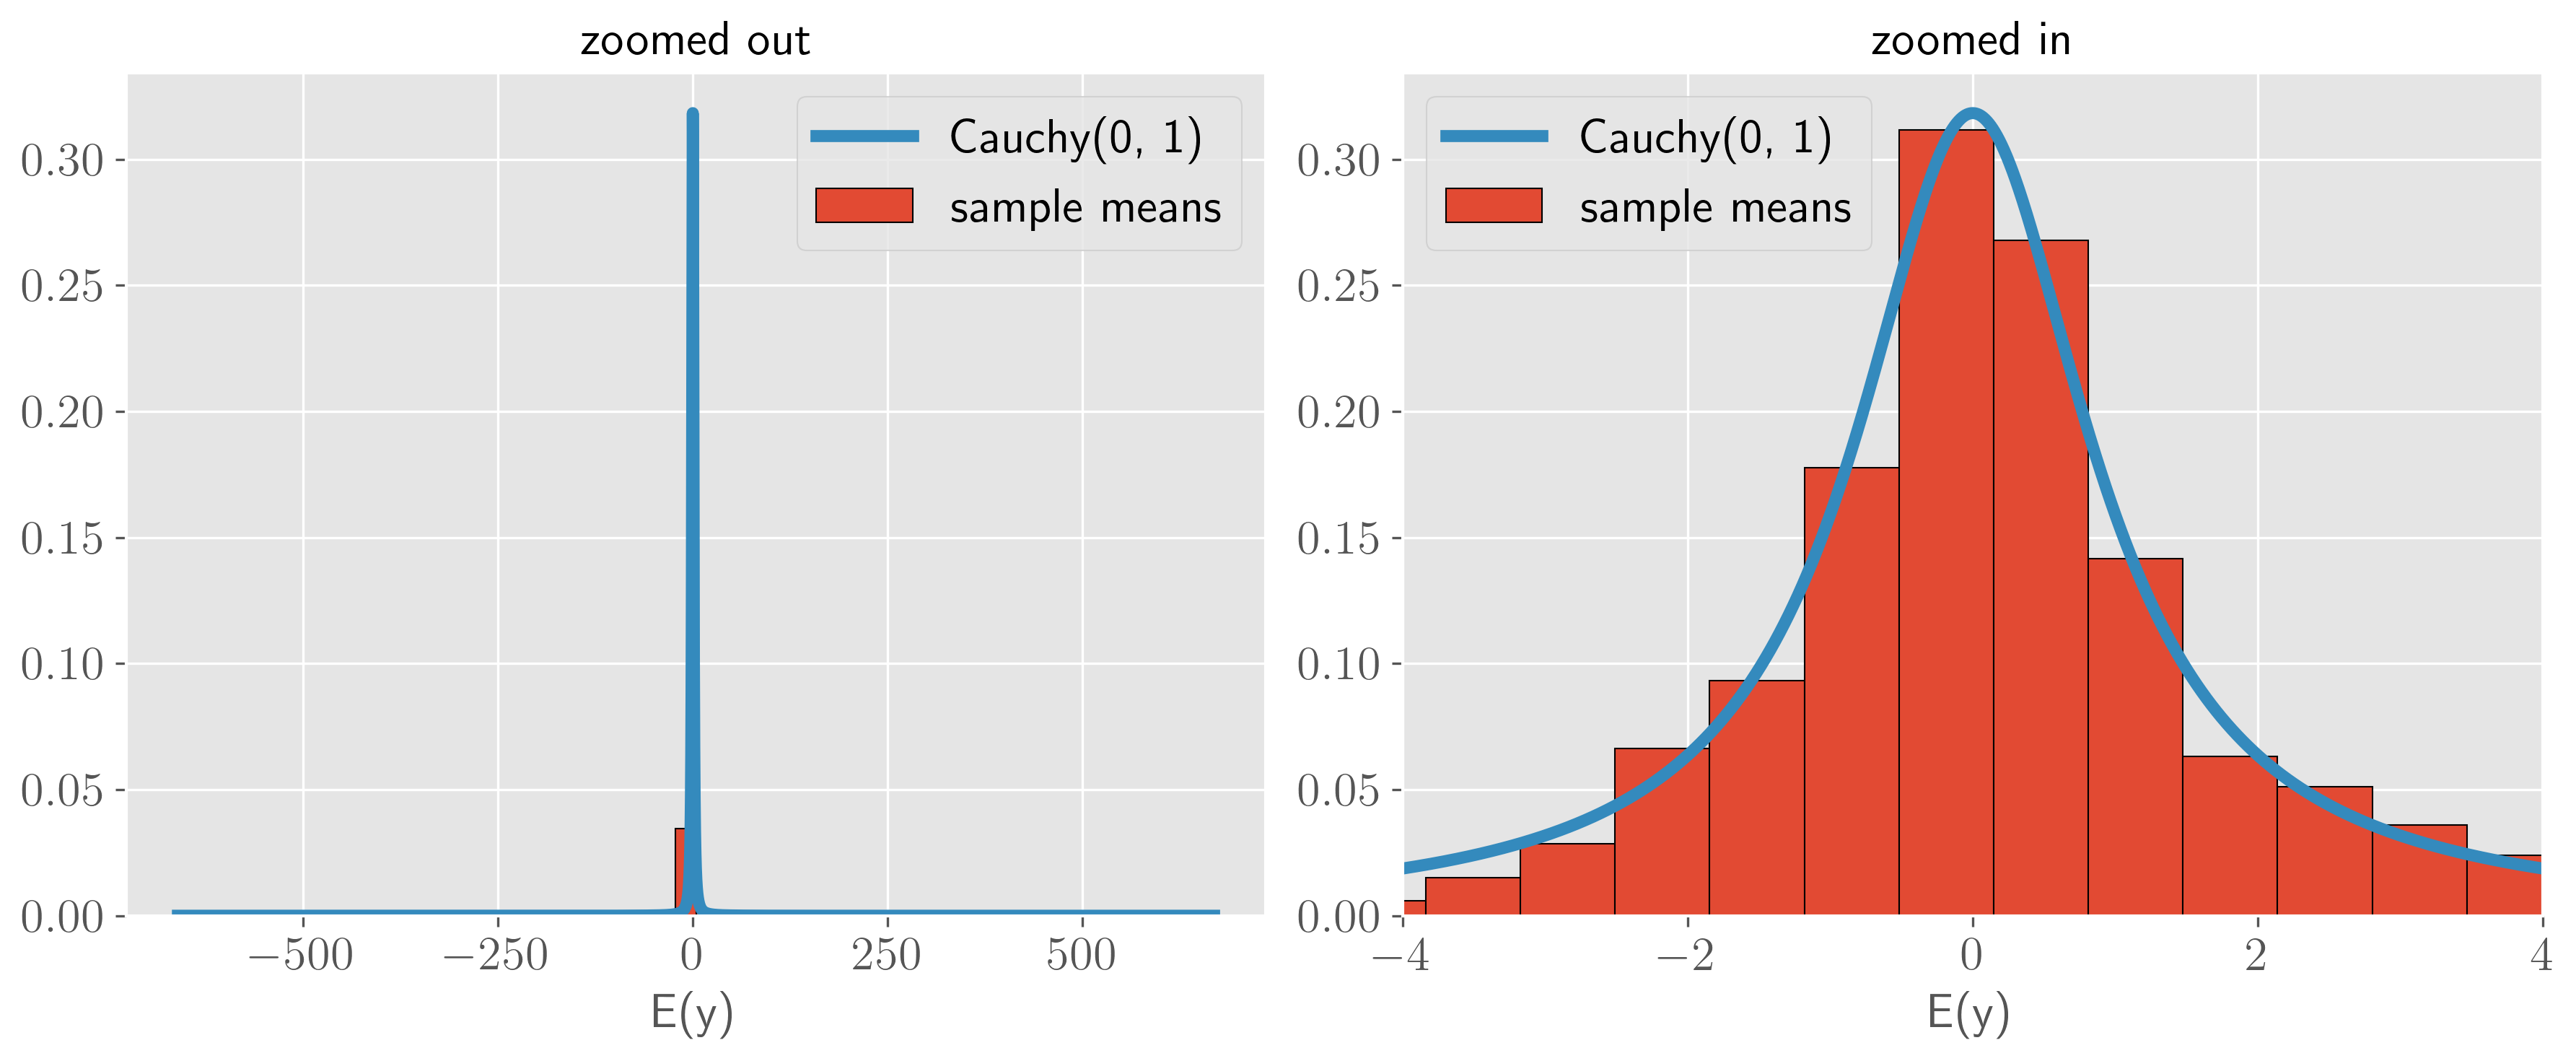
\includegraphics[scale=.55]{homework_2/figures/cauchy_mean.png}
    \caption{Histogram for question (3) (a)}
    \label{fig:my_label}
\end{figure}

\subsection*{Estimate $\theta$ in Cauchy$(\theta, 1)$ using (b) step-wise gradient ascent, (c) Newton-Raphson, and (d) stochastic gradient ascent. }

We need the first and second derivatives of the log likelihood to implement gradient ascent / Newton-Raphson / tochastic gradient ascent. 

\begin{align*} log L(\theta) &= log \prod_{i=1}^n \frac{1}{\pi}\frac{1}{1+(y_i-\theta)^2} \\
&= \sum_{i=1}^n log \frac{1}{\pi}\frac{1}{1+(y_i-\theta)^2} \end{align*}
\begin{align*} \frac{d}{d\theta}log L(\theta) &= \frac{d}{d\theta}\sum_{i=1}^n log \frac{1}{\pi}\frac{1}{1+(y_i-\theta)^2} \\
&=  \sum_{i=1}^n   \frac{2(y_i-\theta)}{1+(y_i-\theta)^2}\end{align*}

\begin{align*} H(\theta) &=\sum_{i=1}^n   \frac{2(y_i-\theta)}{1+(y_i-\theta)^2} \\
&=  \sum_{i=1}^n   \frac{2[(y_i-\theta)^2-1]}{[1+(y_i-\theta)^2]^2} \end{align*}

For gradient ascent and stochastic gradient ascent, we have:

\begin{align*}
    \theta^{(m+1)} = \theta^{(m)} + \gamma \frac{\partial \mathcal{L}(\theta^{(m)})}{\partial \theta}
\end{align*}

For stochastic gradient ascent, we randomly choose a single sample to evaluate the log likelihood at each iteration. For Newton-Raphson (this is the general multidimensional form, we only have one unknown here):

\begin{align*}
    \theta^{(m+1)} = \theta^{(m)} - H(\theta^{(m)})^{-1} \frac{\partial \mathcal{L}(\theta^{(m)})}{\partial \theta}
\end{align*}

Note that the log likelihood was not strictly concave (its second derivative is not strictly negative). Therefore, the optimizations were repeated several times at different starting values and the run resulting in the highest MLE was chosen. The scripts are attached to this homework.

\begin{figure}[!h]
    \centering
    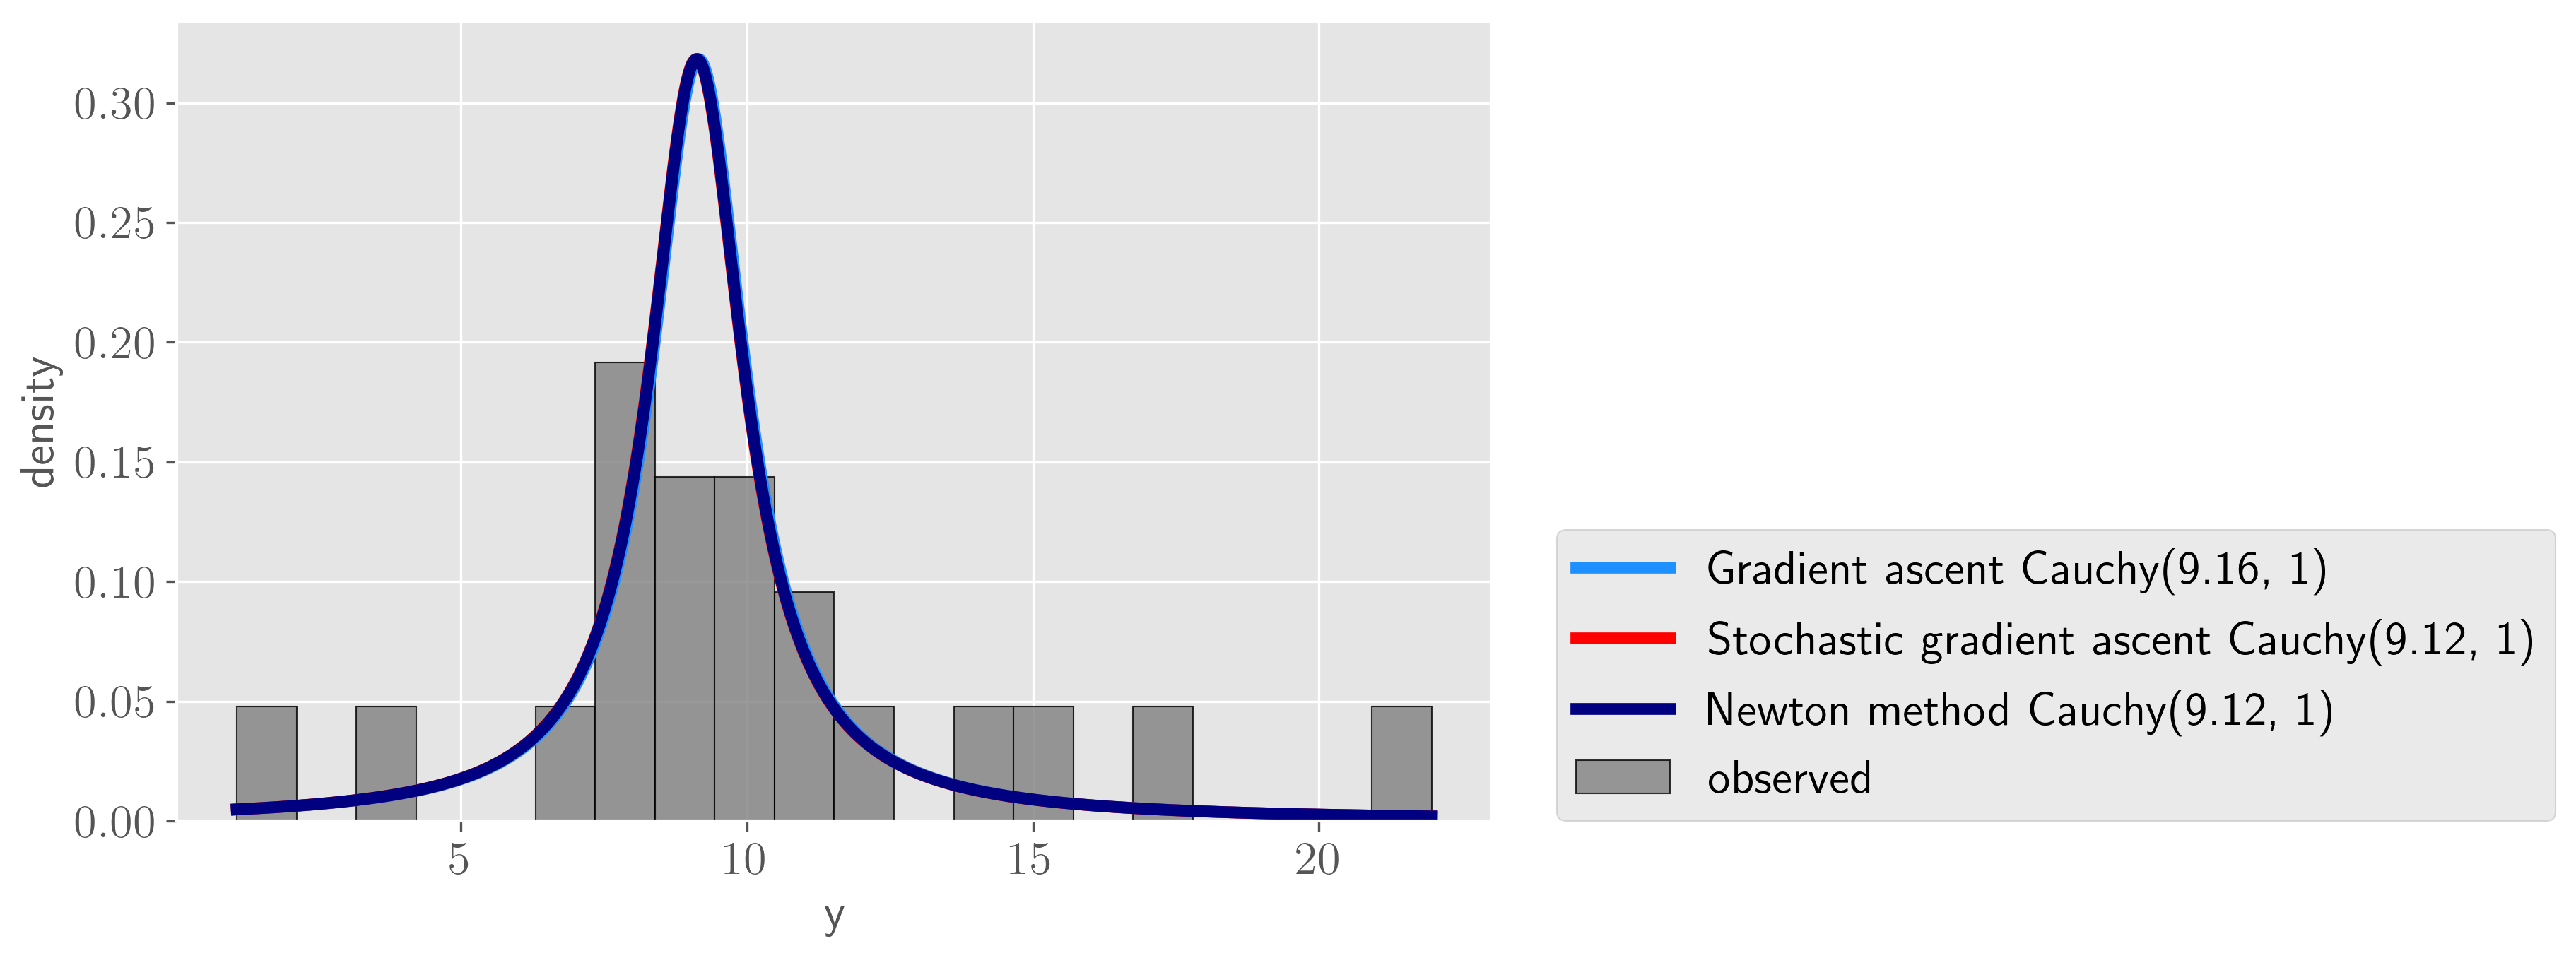
\includegraphics[scale=.55]{homework_2/figures/mle_cauchy.png}
    \caption{Cauchy($\theta$, 1) for the three methods using their $\theta_{MLE}$}
    \label{fig:my_label}
\end{figure}

\begin{figure}[!h]
    \centering
    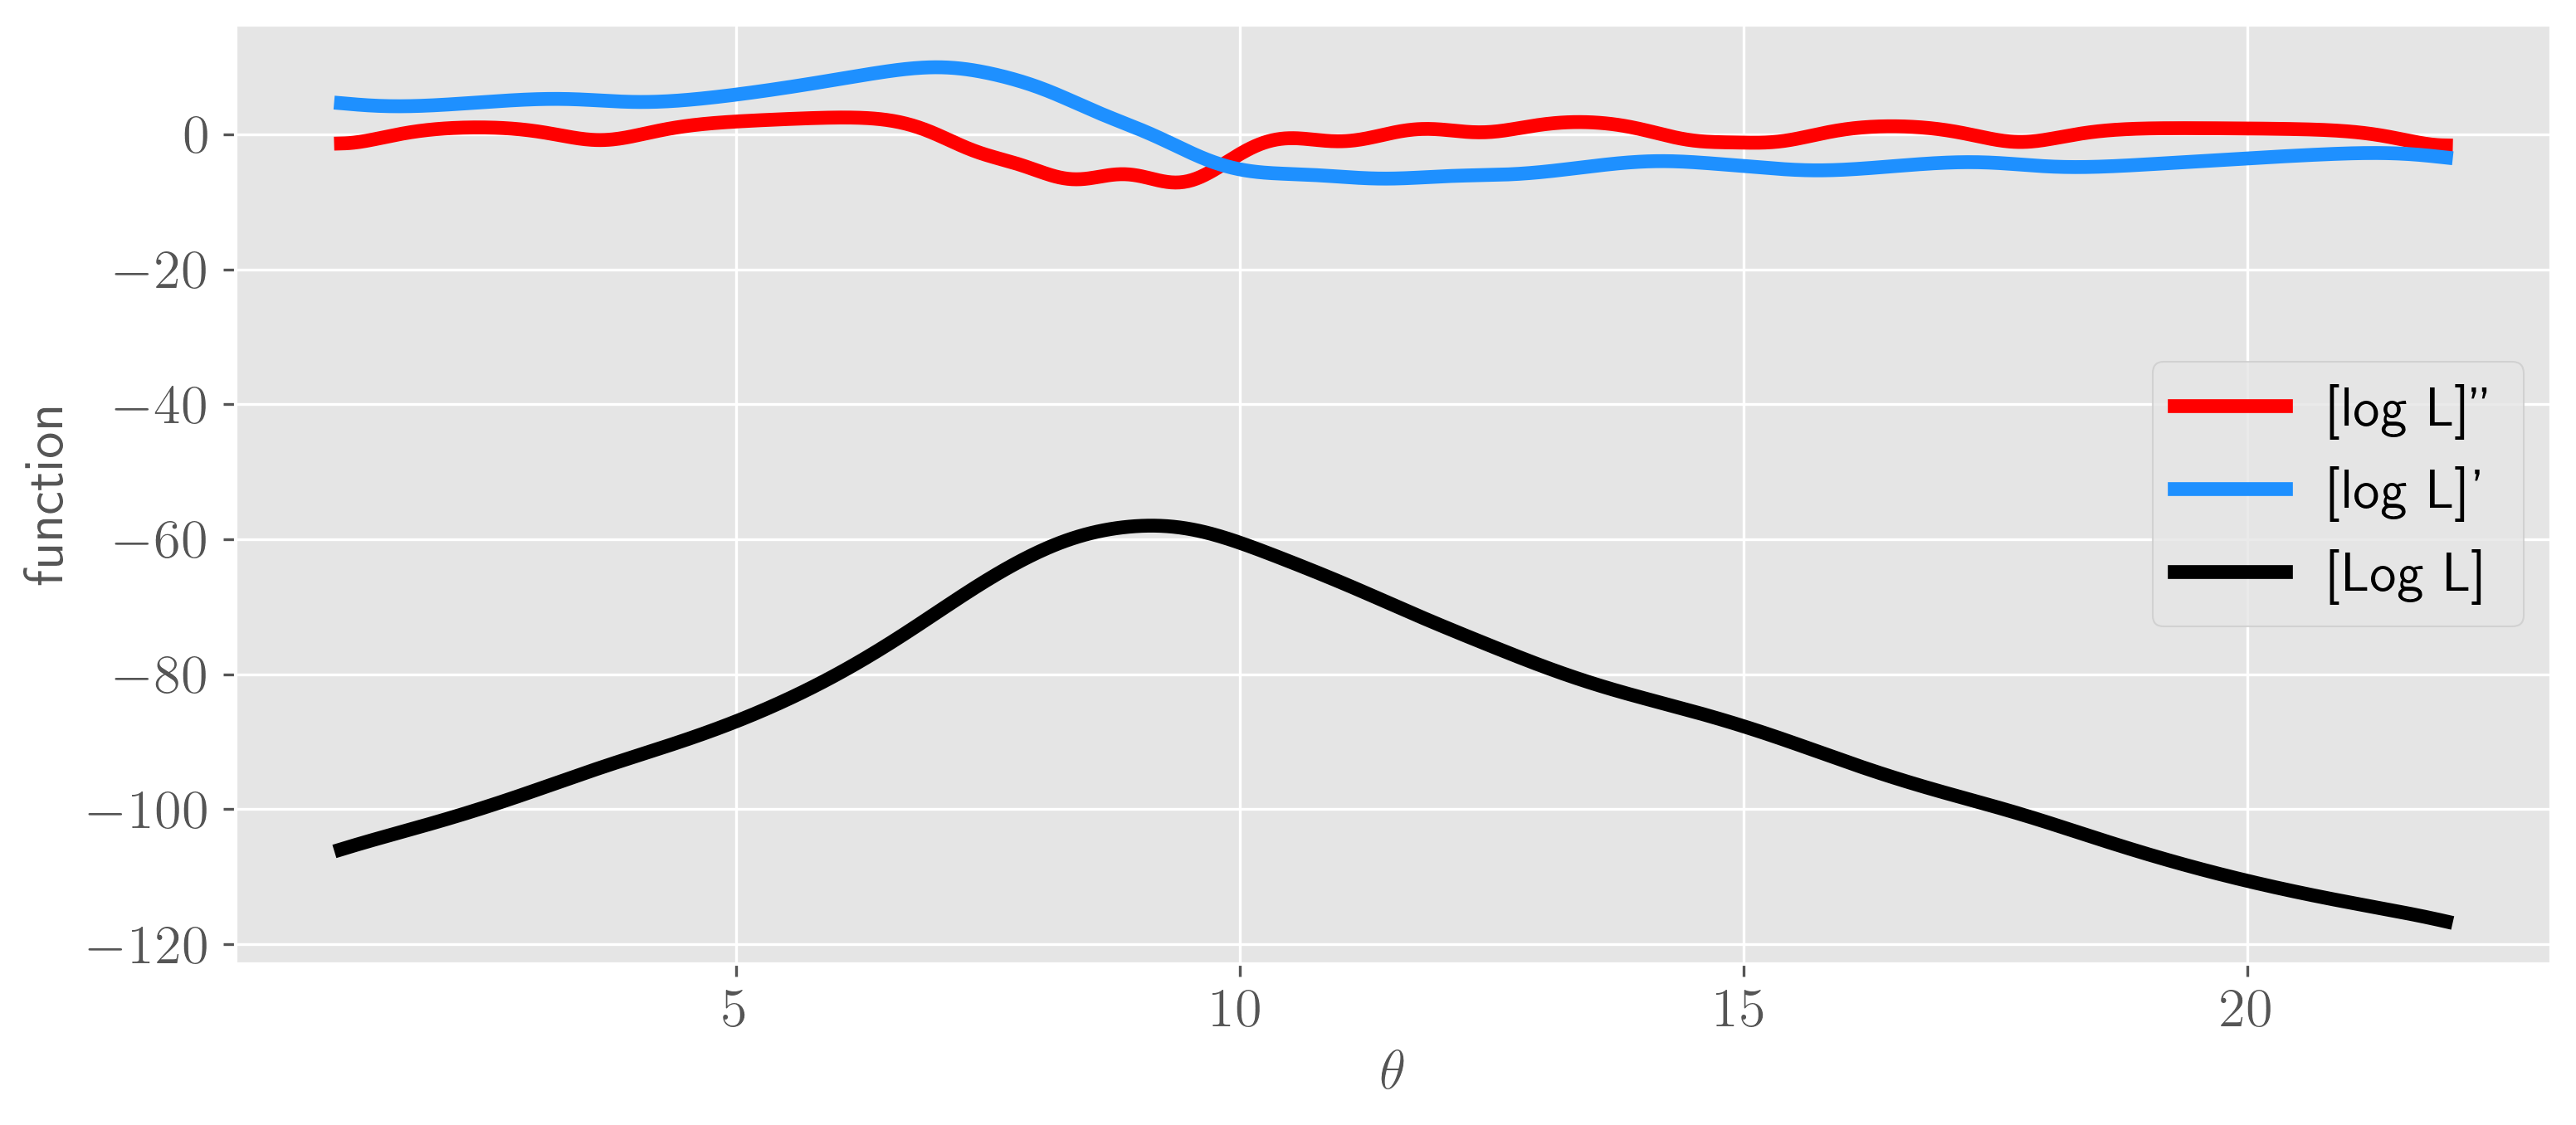
\includegraphics[scale=.55]{homework_2/figures/cauchy_fns.png}
    \caption{Log likelihood and its first and second derivatives}
    \label{fig:my_label}
\end{figure}

\begin{figure}[!h]
    \centering
    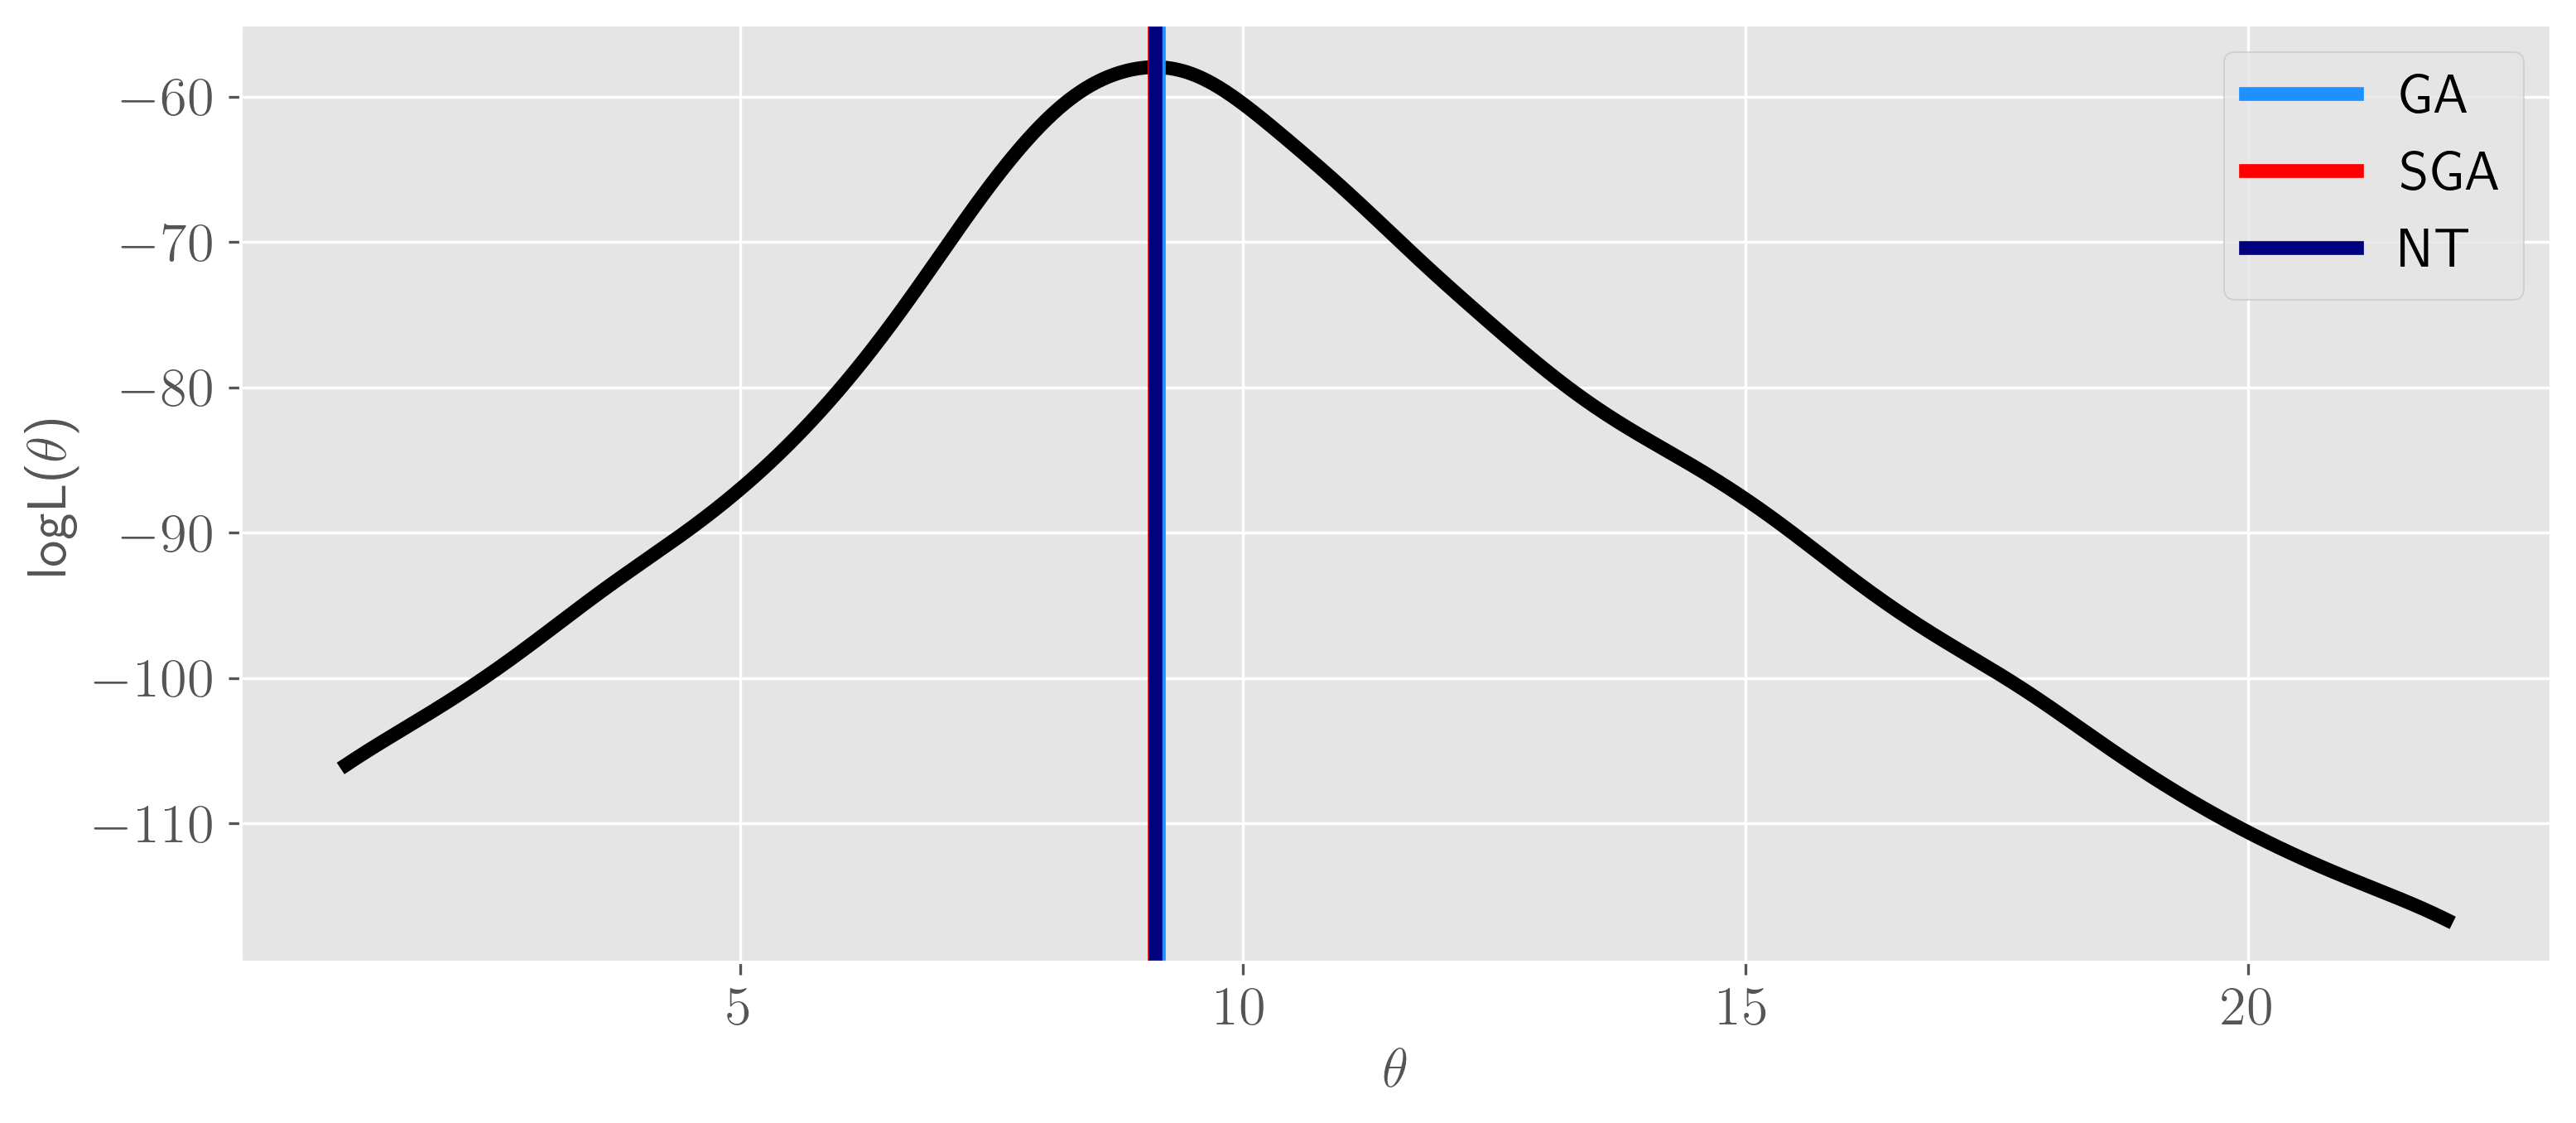
\includegraphics[scale=.55]{homework_2/figures/cauchy_loglike.png}
    \caption{Log likelihood and the $\theta$ values for the three optimizers (they overlap).}
    \label{fig:my_label}
\end{figure}

Newton-Raphson converged in 3 iterations (given the tolerance specified). The two other algorithms took larger number of iterations. In terms of time, Newton-Raphson was also the fastest algorithm to converge.

\subsection*{(4) Let $y_{i,j}$
ind∼ $Normal(\mu_i,\sigma^2)$, $i = 1,...,n$ and $j = 1,...,m$ with $n \xrightarrow[]{} \infty$
but m fixed. Find out the MLEs of $\mu_i$ and $\sigma^2$. Show that  $\hat{\sigma}^2$ MLE is inconsistent for $\sigma^2$. Adjust this estimator to come up with a consistent estimator of  $\sigma^2$.}

We have

\begin{align*}
    L(\mu, \sigma^2) &=  (2\pi \sigma^2)^{-n/2} \text{exp} \left(- \frac{\sum(y_i-\mu)^2}{2\sigma^2}\right)\\
    \mathcal{L}(\mu, \sigma^2) &= -\frac{n}{2}log(2\pi)  -\frac{n}{2}log(\sigma^2)  -\frac{1}{2\sigma^2}\sum(y_i-\mu)^2
\end{align*}

and 

\begin{align*}
    \frac{\partial \mathcal{L}(\mu, \sigma^2)}{\partial \mu} &= 0 \\
    -\frac{1}{2\sigma^2} \sum -2(y_i-\mu)&= 0 \\
     \sum y_i-n\mu&= 0 \\
     \mu&= \bar{y} \\
\end{align*}

\begin{align*}
    \frac{\partial \mathcal{L}(\mu, \sigma^2)}{\partial \sigma^2} &= 0 \\
    -\frac{n}{2\sigma^2} + \frac{1}{2\sigma^4}\sum (y_i - \mu)^2&= 0 \\
     -\frac{n}{2} + \frac{1}{2\sigma^2}\sum (y_i - \mu)^2&= 0 \\
     -\sigma^2n +\sum (y_i - \mu)^2&= 0 \\
     \sigma^2 &= \sum (y_i - \mu)^2 / n \\
\end{align*}

In practice we would replace $\mu$ with $\bar{y}$. But

\begin{align*}
    E(\sigma^2_{MLE}) &= E\left(\sum (y_i - \bar{y})^2 / n\right)\\
    &= \frac{1}{n} E\left(\sum y_i^2 - 2\bar{y} \sum y_i + \bar{y}n \right)\\
    &= \frac{1}{n} E\left( y_i^2 - 2\bar{y}^2n + \bar{y}^2n \right)\\
     &= \frac{1}{n} E\left( \sum y_i^2 - \bar{y}^2n \right)\\
      &= \frac{1}{n} E\left( \sum y_i^2 - \bar{y}^2n \right)\\
       &=  E( y^2) - E(\bar{y}^2)\\
          &=  var(y) + E(y)^2 - var(\bar{y}) - E(\bar{y})^2 \\
            &=  var(y)  - var(\bar{y}) \\
              &=  var(y)  - var(y)/n \\
               &=  \frac{(n-1)\sigma^2}{n}\\
\end{align*}
So, a better estimator is $\sum (y_i - \mu)^2 / (n-1) $.

\subsection*{(5) For $y_1,...,y_n \sim Uniform(0, 
\theta)$, show that $ z_n = \frac{n(\theta-\hat{\theta}_{MLE})}{\theta} \xrightarrow[]{D} E$, where E is exponential. Design a simulation study illustrating this nice result.}

We have, for $y \in [0, \theta]$

\begin{align*}
    f(y) &= 1/\theta \\ 
    L(\theta) &= 1/ \theta ^n\\
\end{align*}

In order to maximize $L(\theta)$, it is obvious that $\theta = max(y_i)$ because if it is less than $ max(y_i)$, samples will be left out (which  will have probability 0).

\begin{align*}
    P\left(\frac{n[\theta-\hat{\theta}_{MLE}] }{\theta} \leq t\right) &= 1 -  P\left(\frac{n[\theta-\hat{\theta}_{MLE}] }{\theta}  \geq t\right)\\
    &= 1 -  P\left(\hat{\theta}_{MLE}  \leq \frac{\theta[t-n]}{n} \right)\\
     &= 1 -  P\left(\hat{\theta}_{MLE}  \leq \frac{\theta[t-n]}{n} \right)\\
      &= 1 -  P\left(max(y)  \leq \frac{\theta[t-n]}{n} \right)\\
       &= 1 -  \prod P\left(y_i  \leq \frac{\theta[t-n]}{n} \right)\\
        &= 1 -  \left( \frac{\frac{\theta[t-n]}{n}}{\theta} \right)^n\\
          &= 1 -  (1-t/n)^n\\
\end{align*}


\begin{figure}[!h]
    \centering
    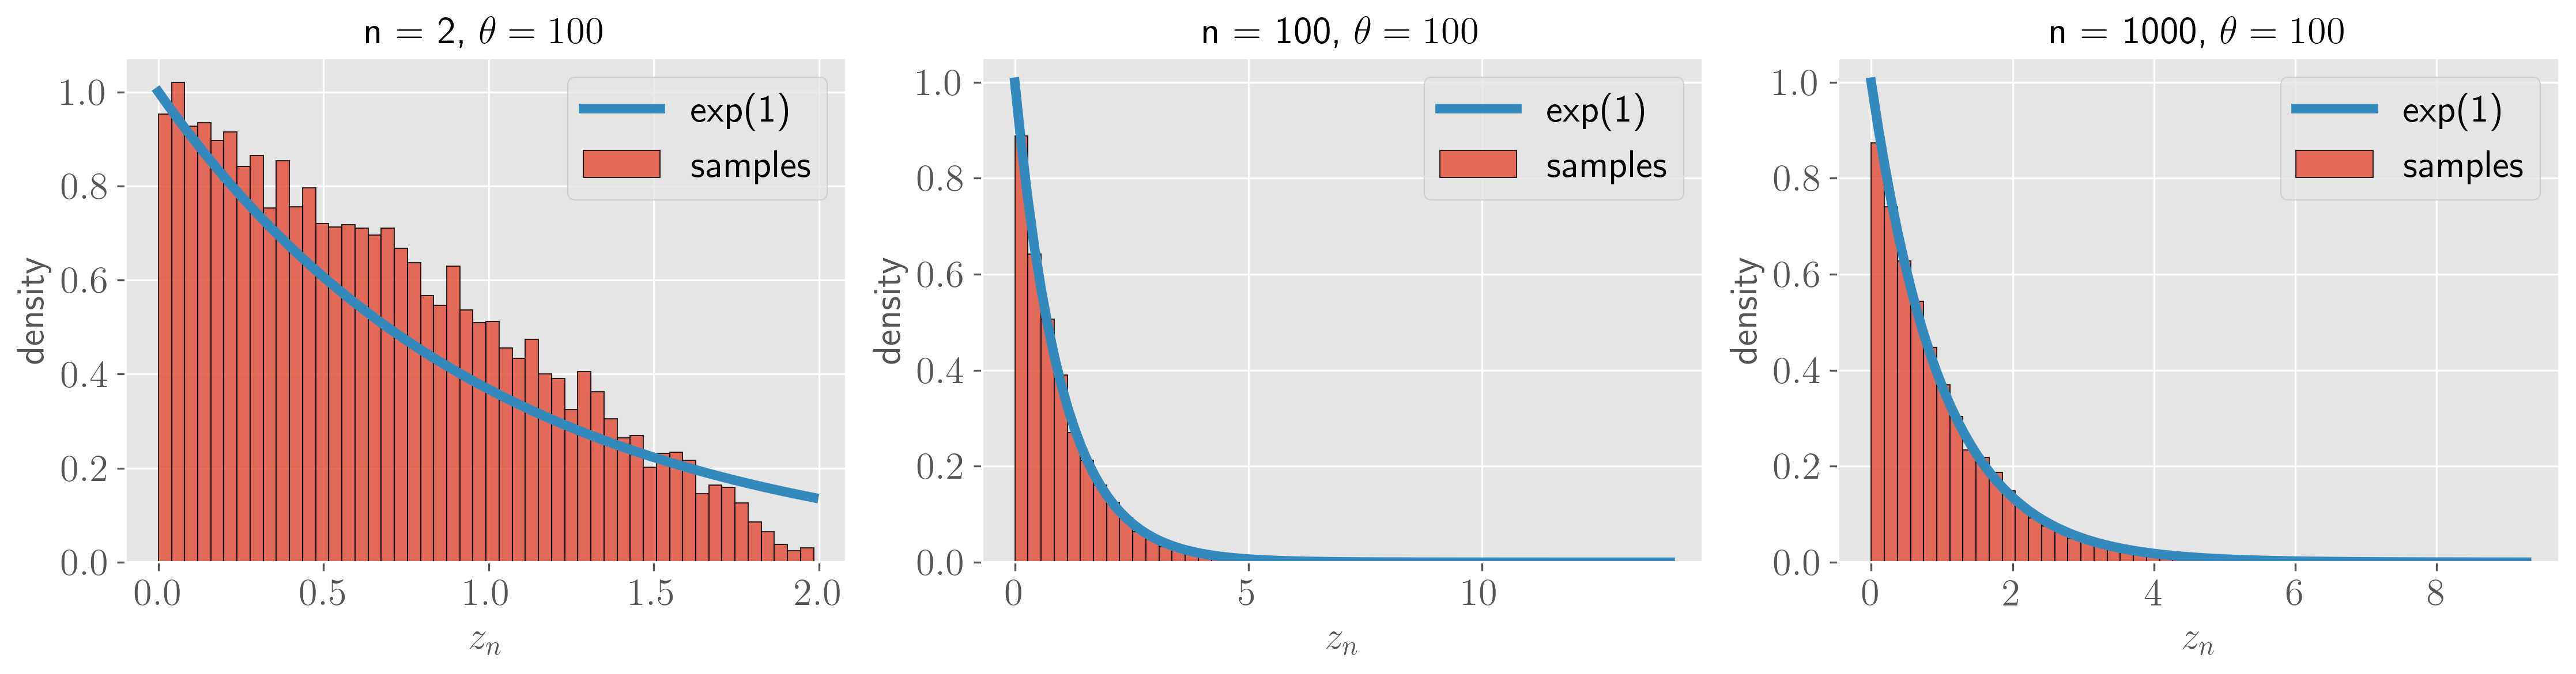
\includegraphics[scale=.4]{homework_2/figures/uniform.png}
    \caption{Simulation illustrating proof shown above.}
    \label{fig:my_label}
\end{figure}

\subsection*{(6)  Using the method of maximum likelihood, fit a Weibull distribution to these data . Also find an approximate 90\% joint confidence region for the parameters $(k, \lambda)$. Supplement your analysis with appropriate plots.}

Gradient ascent did not converge well for this, so I used Newton-Raphson. The log likelihood, first derivatives and observed information were:

\begin{align*}
    \mathcal{L}(k, \lambda) &= \sum \text{log} \frac{k}{\lambda} \left(\frac{x_i}{\lambda}\right)^{k-1}e^{-(x_i/\lambda)^k}\\
    &=  n\text{log} k - n\text{log} \lambda + (k-1)\sum \text{log}(x_i/\lambda) -\sum(x_i/\lambda)^k
\end{align*}


\begin{align*}
   \frac{\partial}{\partial k}\mathcal{L}(k, \lambda) &=  \frac{\partial}{\partial k}\mathcal{L} n\text{log} k - n\text{log} \lambda + (k-1)\sum \text{log}(x_i/\lambda) -\sum(x_i/\lambda)^k\\
   &= n/k + \sum \text{log}(x_i/\lambda)-\sum (x_i/\lambda)^k \text{log} (x_i/\lambda)
\end{align*}

\begin{align*}
   \frac{\partial}{\partial \lambda}\mathcal{L}(k, \lambda) &=  \frac{\partial}{\partial \lambda} n\text{log} k - n\text{log} \lambda + (k-1)\sum \text{log}(x_i/\lambda) -\sum(x_i/\lambda)^k\\
   &= -nk/\lambda + k/\lambda \sum (x_i/\lambda)^k
\end{align*}

The observed information was:



\begin{center}
    \begin{bmatrix}

n/k^2 + \sum(y_j /\lambda)^k\{\text{log}(y_j /\lambda)\}^2

& \lambda^{-1} \sum[1 - (y_j - \lambda)^
k\{1 + k \text{log}(y_j /\lambda)\}] \\
\lambda^{-1} \sum[1 - (y_j -\lambda)^k\{1 + k log(y_j /\lambda)\}]
&k(k + 1)/\lambda^2 \sum(y_j /\lambda)^k - nk\lambda^{-2}
\end{bmatrix}
\end{center}

Using Newton, I found $(\lambda, k) = (181.4, 5.98)$. The plots below show the log likelihood and the Weibull pdf with the mle parameters and observed data.


\begin{figure}[!h]
    \centering
    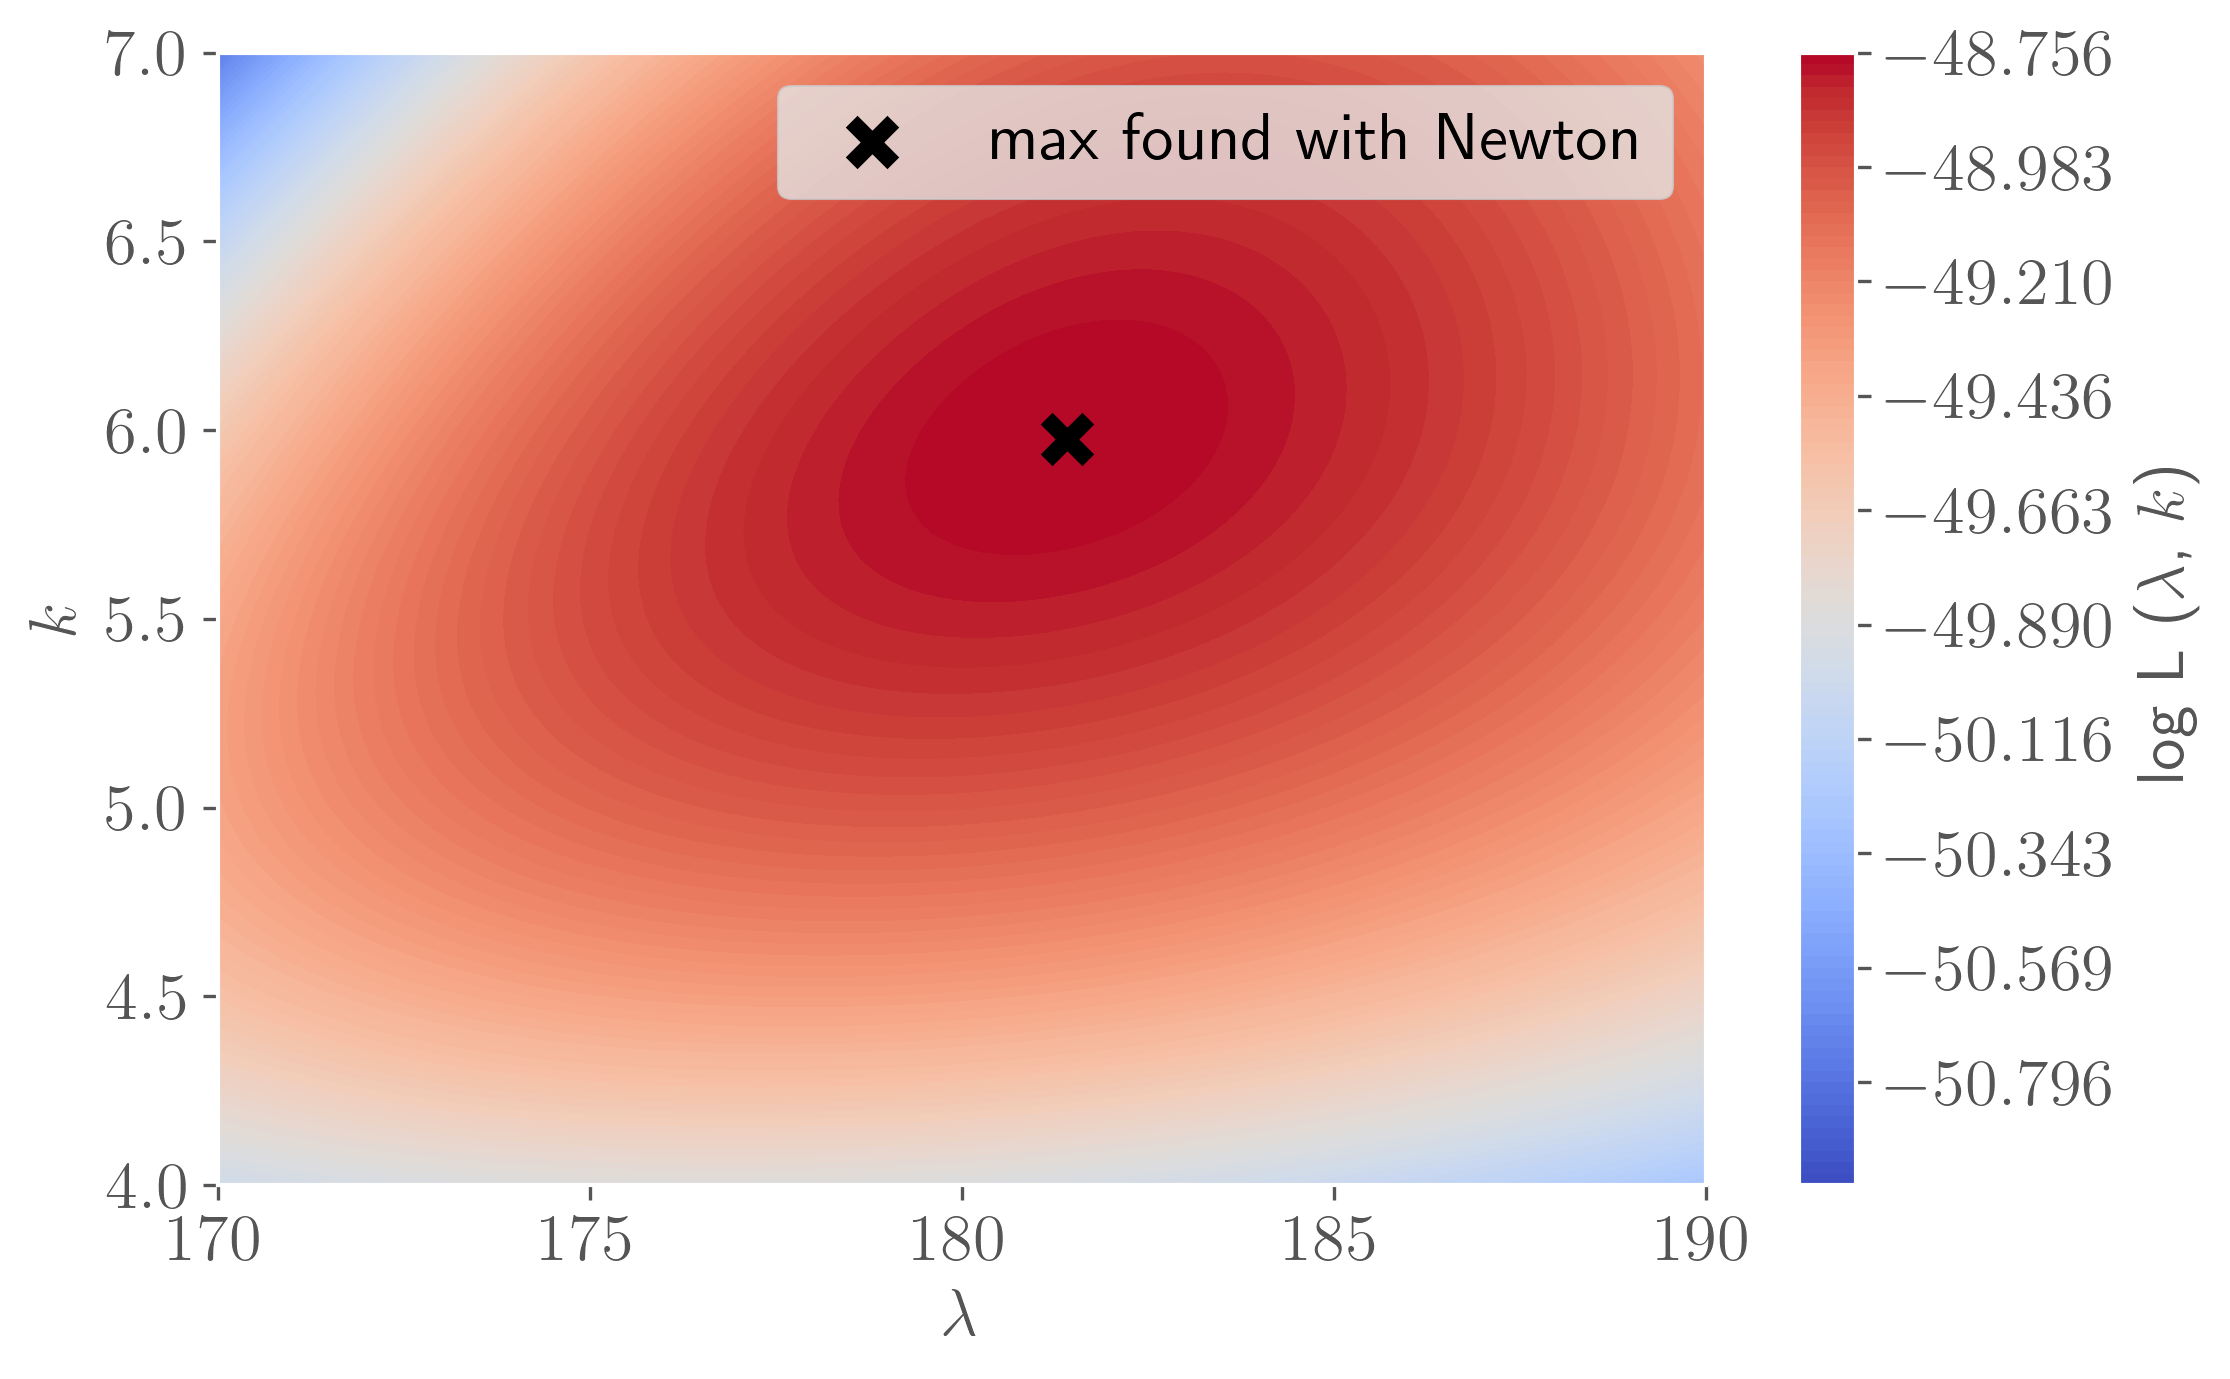
\includegraphics[scale=.55]{homework_2/figures/mle_weibull.png}
    \caption{Log likelihood and mle parameters}
    \label{fig:my_label}
\end{figure}

\begin{figure}[!h]
    \centering
    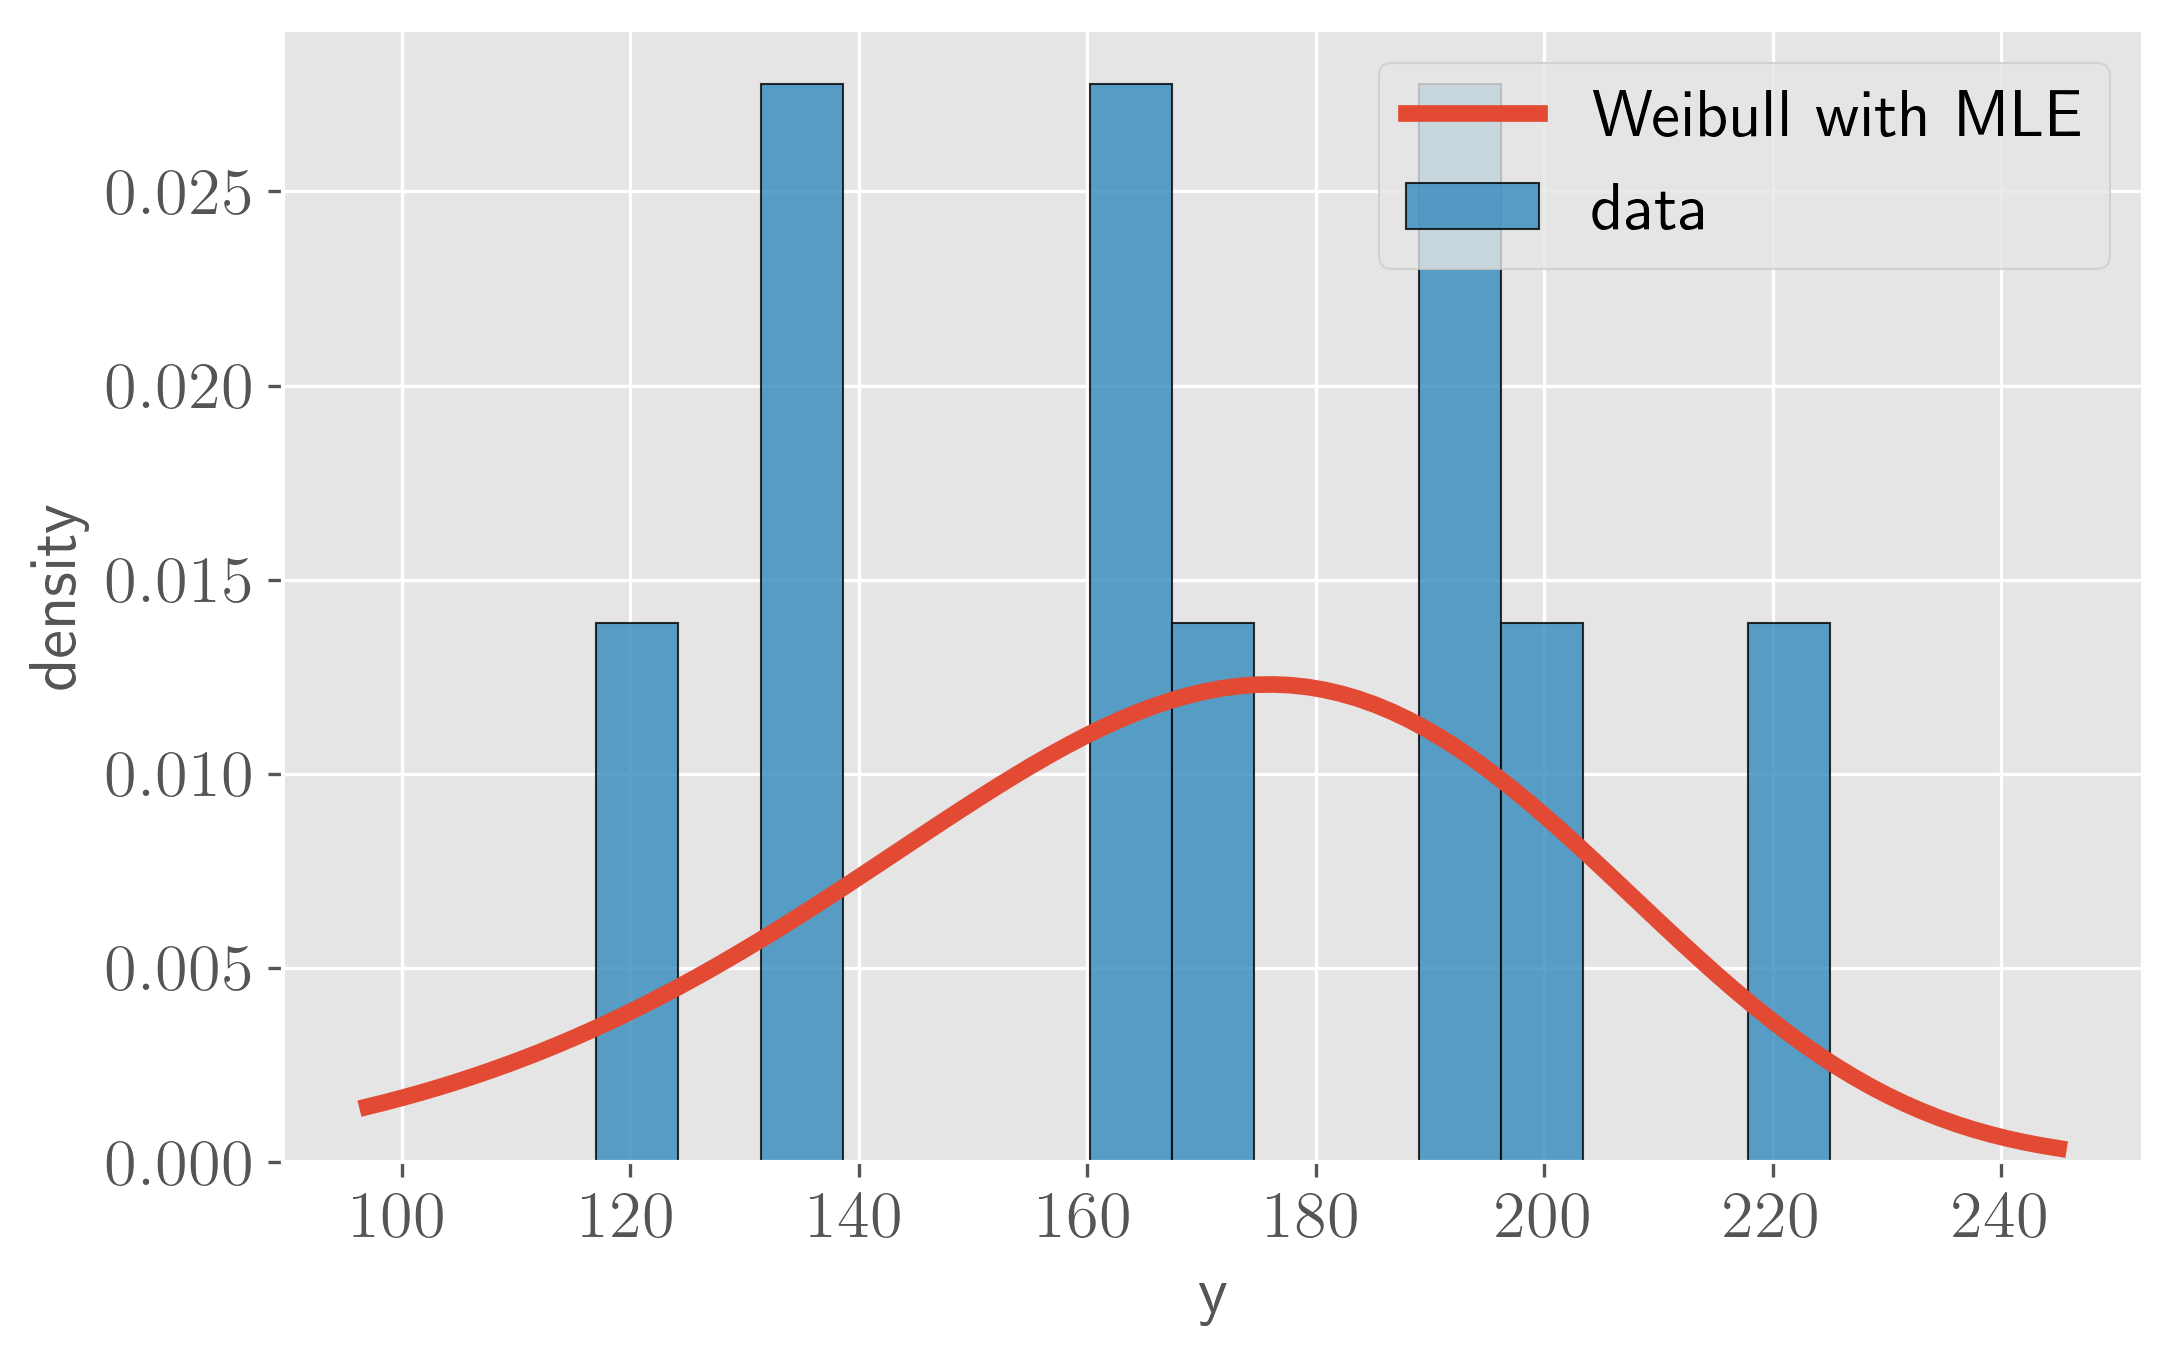
\includegraphics[scale=.55]{homework_2/figures/weibull_data_fit.png}
    \caption{Histogram of the data and density found using MLE.}
    \label{fig:my_label}
\end{figure}

To calculate the standard error, the observed information can be used as an approximation. We also use the fact that $(\theta_{MLE} - \theta)^T J(\theta_{MLE})(\theta_{MLE} -\theta) \approx \chi^2_2$. $\chi^2_{\alpha}$ for $alpha = 0.1$ (right tailed) is 4.605. J is evaluated at $\theta_{MLE}$. We then have:

\begin{align*}
    P[(\theta_{MLE} - \theta)^T J(\theta_{MLE})(\theta_{MLE} - \theta) \leq 4.605] = 0.90
\end{align*}

So we want the ellipse satisfying:

\begin{align*}
    (\theta_{MLE} - \theta)^T J(\theta_{MLE})(\theta_{MLE} - \theta) = 4.605
\end{align*}
To draw this ellipse, we use the Cholesky decomposition of $J$.

\begin{align*}
     & (\theta_{MLE} - \theta)^T J(\theta_{MLE})(\theta_{MLE} - \theta)\\
     &=  (\theta_{MLE} - \theta)^T LL^T(\theta_{MLE})(\theta_{MLE} - \theta)\\
       &=  [L^T(\theta_{MLE} - \theta)^T] [L^T(\theta_{MLE})(\theta_{MLE} - \theta)]
\end{align*}

First we take linearly spaced angles $\phi$ between 0 and $2\pi$ and transform them using:

\begin{align*}
    X = \theta_{MLE} + 4.605^{1/2} L^{-T} [cos \phi, sin\phi]
\end{align*}
This results in the figure shown below.



\begin{figure}[!h]
    \centering
    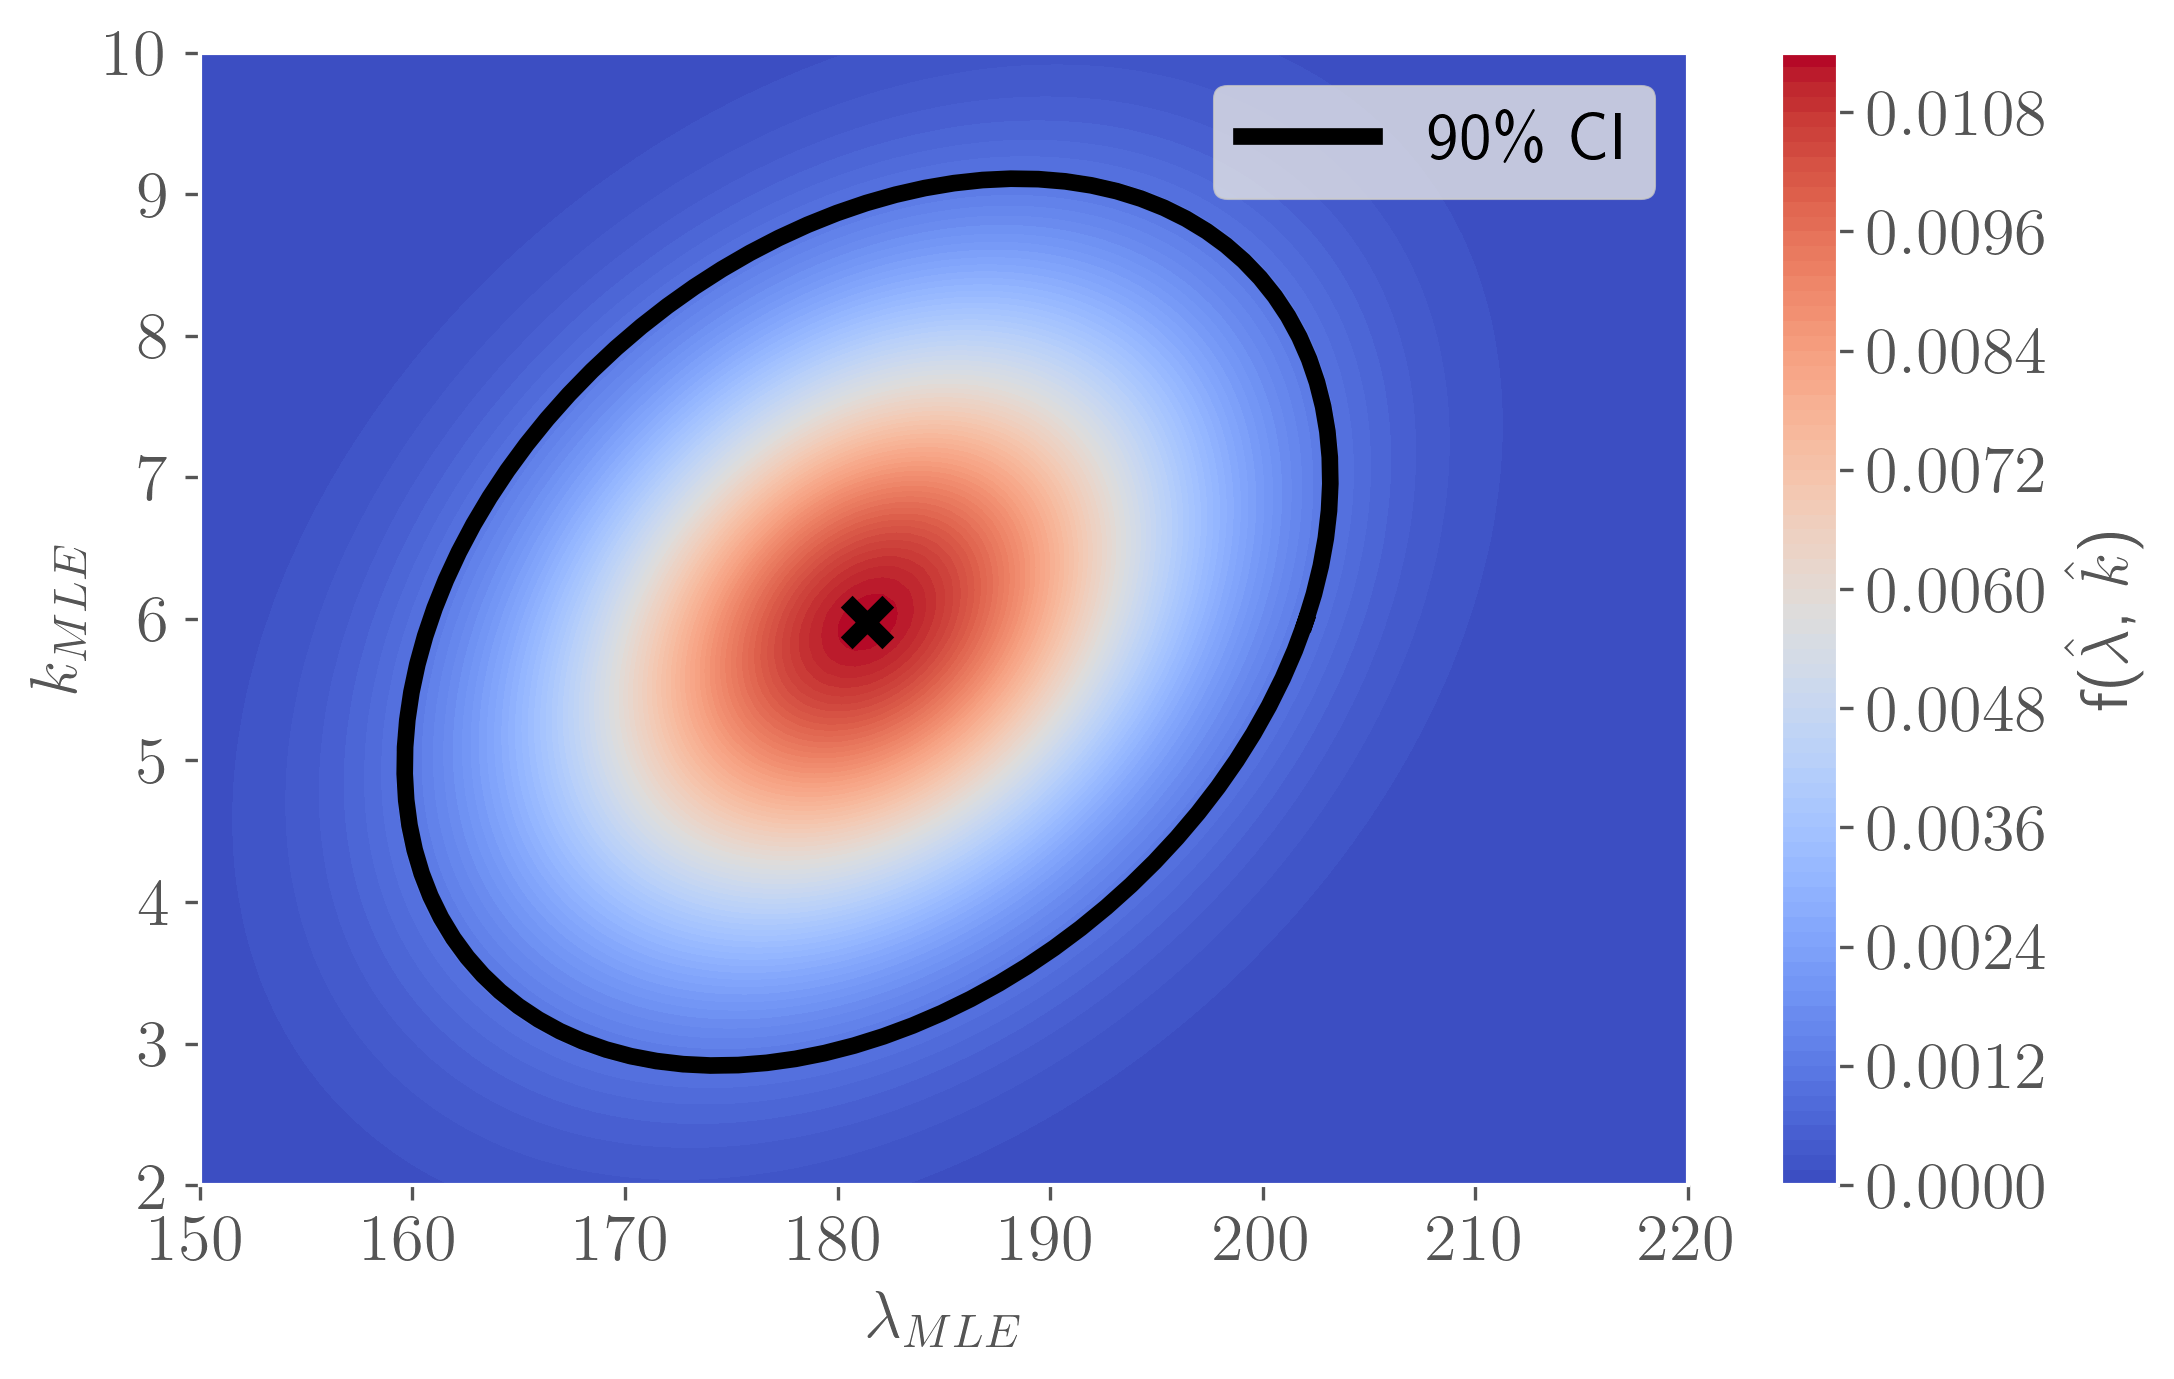
\includegraphics[scale=.55]{homework_2/figures/weibull_se.png}
    \caption{Standard error ellipse for the mle parameters.}
    \label{fig:my_label}
\end{figure}

\subsection*{(7) For a Weibull$(k,\lambda$) distribution, design a
simulation study to show that \\ $(\theta_{MLE})^TJ)(\theta_{MLE})\xrightarrow[]{} \chi^2_2$ and $W(\theta) \xrightarrow[]{}  \chi^2_2$}.

I built the simulations using $(\lambda, k) = (0.5, 2)$ and re-used the Newton-Raphson code I had used for the previous question. I ran it for 1,000 iterations with $5,000$ samples in each. The plots below show that that  $(\theta_{MLE})^TJ)(\theta_{MLE})\xrightarrow[]{} \chi^2_2$ and $W(\theta) \xrightarrow[]{}  \chi^2_2$.



\end{document}